\documentclass{article}
\usepackage{algpseudocode}
\usepackage[ruled]{algorithm}
\usepackage{url}
\usepackage{framed}
\usepackage{amsfonts,amsmath,amsthm,amssymb}
\usepackage{graphicx}
\usepackage{url}
\usepackage{color}
\usepackage{geometry}

\geometry{margin=1.2in}

\newcommand {\mean} {\ensuremath {\mathop{\mathrm{mean}}}}
\newcommand {\median} {\ensuremath {\mathop{\mathrm{median}}}}
\newcommand {\N} {\ensuremath {\mathcal{N}}}
\newcommand {\IE} {\ensuremath {\mathbb{E}}}
\newcommand {\cov} {\ensuremath {\mathop{\mathrm{cov}}}}
\newcommand {\BEL} {\ensuremath {\mathop{\mathrm{BEL}}}}

\newtheorem{lemma}{Lemma}

\title{Doing Better Than UCT: \\ Rational Monte Carlo Sampling in Trees}
\author {David Tolpin, Solomon Eyal Shimony \\
Department of Computer Science, \\
Ben-Gurion University of the Negev, Beer Sheva, Israel \\
\{tolpin,shimony\}@cs.bgu.ac.il}

\begin{document}

\maketitle

\begin{abstract}
UCT, a state-of-the art algorithm for Monte Carlo tree sampling
(MCTS), is based on UCB, a sampling policy for the Multi-armed Bandit
Problem (MAB) that minimizes the accumulated regret. However, MCTS
differs from MAB in that only the final choice, rather than all arm
pulls, brings a reward, that is, the simple regret, as opposite to the
cumulative regret, must be minimized. This ongoing work aims at applying
meta-reasoning techniques to MCTS, which is non-trivial.
We begin by introducing policies for
multi-armed bandits with lower simple regret than UCB, and an
algorithm for MCTS which combines cumulative and simple regret
minimization and outperforms UCT. We also develop a sampling scheme loosely based
on a myopic version of perfect value of information.
Finite-time and asymptotic analysis of
the policies is provided, and the algorithms are compared empirically.
\end{abstract}


\section{Introduction and definitions}

Monte-Carlo tree sampling, and especially a version based on the
UCT formula \cite{Kocsis.uct} appears in numerous search applications,
such as \cite{Eyerich.ctp}. Although these methods are shown to be successful empirically,
most authors appear to be using the UCT formula ``because it has been shown
to be successful in the past'', and ``because it does a good job of
trading off exploration and exploitation''. While the latter statement may be
correct for the multi-armed bandit and for the UCB method \cite{Auer.ucb},
we argue that it is inappropriate for search. The problem is not that
UCT does not work; rather, we argue that a simple reconsideration from basic
principles can result in schemes that outperform UCT. This is demonstrated both
theoretically and empirically.

In the Multi-armed Bandit problem we have a set of $K$ arms. Each arm can be pulled
multiple times. When the $i$th arm is pulled, a random reward $X_i$
from an unknown stationary distribution is returned.  The reward is 
bounded between 0 and 1. 

The simple regret of a sampling policy for the Multi-armed Bandit
Problem is the expected difference between the best expected reward
$\mu_*$ and the expected reward $\mu_j$ of the arm with the best sample mean
$\overline X_j=\max_i\overline X_i$:
\begin{equation}
\label{eq:simple-regret}
\IE[R]=\sum_{j=1}^K\Delta_j\Pr(\overline X_j=\max_i\overline X_i)
\end{equation}
where $\Delta_j=\mu_*-\mu_j$.
Strategies that minimize the simple reward are called pure exploration
strategies \cite{Bubeck.pure}.

Such strategies are used to select the best arm, and, by extension,
the best action in Monte Carlo tree search. Monte Carlo tree search is
used to solve Markov Decision Processes (MDP) approximately. An MDP is
defined by the set of states $S$, the set of actions $A$, the
transition table $T(s, a, s')$, the reward table $R(s, a, s')$, the
initial state $s$ and the goal state $t$: $(S, A, T, R, s, t)$
\cite{Russell.aima}.  Monte Carlo tree search explores an MDP by
\emph{rollouts}---trajectories from the current state to a state in
which a termination condition is satisfied (either the goal state, or
a cutoff state for which the reward is evaluated
approximately). The UCB algorithm (that attempts to minimize the cumulative regret)
\cite{Auer.ucb} had been extended into the tree search sampling scheme
known as UCT \cite{Kocsis.uct}.

UCT-driven search achieves good results in many search problems. At each
search step, the algorithm allocates Monte Carlo rollouts to choose
the best action, thereby (approximately) minimizing the cumulative regret. 
The core issue is that in search (especially for adversarial search
and for ``games against nature'' - optimizing behavior under uncertainty) the goal is typically
to either find a good (or optimal) strategy, or even to find the best first
action of such a policy. Once such an action is discovered, it is not beneficial
to further sample that action, ``exploitation'' is thus meaningless for
search problems. Finding a good first action is closer to the pure exploration
variant, as seen in the selection problem \cite{Bubeck.pure,TolpinShimony.blinkered}. In the selection
problem, it is much better to minimize the {\em simple} regret.
However, the simple and the cumulative regret cannot be minimized simultaneously;
moreover, \cite{Bubeck.pure} shows that in many cases the smaller the
cumulative regret, the greater the simple regret.


UCT performance can thus be improved by combining UCB with a sampling
scheme that minimizes the simple regret of selecting an action at the
current root node. Indeed, the algorithm must select an action with
the minimum regret \emph{given the assumption that after performing the selected action
the algorithm performs optimally}, which corresponds to maximizing the
value of partial information \cite{Russell.aima}. Therefore, an
improved allocation scheme would
\begin{itemize}
\item maximize the value of partial
information by sampling actions to
minimize the \textbf{simple} regret
of the selection at the current root node, and
\item as the goal of sampling in deeper tree nodes is estimating the value of
a node, rather than selection, it makes sense to
minimize the \textbf{cumulative} regret of the rollouts from the second
step onwards. 
\end{itemize}

The ultimate goal of this ongoing work is ``optimal'' sampling
in the meta-reasoning sense. Nevertheless, this task is daunting for
the following reasons:
\begin{itemize}
\item Defining the cost of a sample is not easy, and even if we simply use time-cost
as an approximation, we get an intractable meta-reasoning problem.
\item Applying the standard myopic and subtree independence assumptions, we run into
serious problems. Even in the standard selection problem \cite{TolpinShimony.blinkered}, we get a non-concave
utility function and premature stopping of the algorithm. This is due to the fact
that the value of information of a single measurement (analogous
to a sample in MCTS) is frequently less than its
time-cost, even though this is not true for multiple measurements.
When applying the selection problem to MCTS, the situation is exacerbated. 
The utility of an action is usually bounded, and thus in many cases a single sample
may be insufficient to change the current best action, {\em regardless} of its
outcome. As a result, we frequently
get a {\em zero} ``myopic'' value of information for a single sample.
\end{itemize}

As the ultimate task is extremely difficult
to achieve, and even harder to analyze, we begin with
simple schemes more amenable to analysis. We then
develop a crude value of information (VOI)
based scheme. Although the latter is a somewhat ad-hoc attempt to
estimate value of information of a sample, it already appears (empirically) to do
better than UCT as well as better than all the simpler schemes we propose.

\section{Main Results}

\subsection{Doing better than UCB}

\begin{enumerate}
\item The $\varepsilon$-greedy allocation scheme has exponential convergence
rate of the simple regret $\IE r$:
\begin{equation}
  \IE r_\varepsilon\le\sum_{j=1}^K\Delta_j\left(\frac {n\varepsilon} K + \frac {4\sqrt e}
{\Delta_j^2}\right)e^{-\Delta_j^2n\varepsilon/8K}
\end{equation}
\item The UCB allocation scheme exhibits polynomial convergence
rate:
\begin{equation}
\IE r_{ucb} \le 2\sum_{j=1}^K \Delta_jn^{\frac {-\alpha \Delta_j^2} 8}
\end{equation}
\item A tighter upper regret bound for the $\varepsilon$-greedy allocation scheme depends on
$\varepsilon$. The lowest bound is
achieved for $\varepsilon=\frac 1
2$, and for a large number of arms the bound for the $\frac 1 2$-greedy scheme approaches the square of the
bound for uniform sampling.

\item Another improved allocation scheme for minimizing the simple regret,
called \textbf{UQB} here, is obtained by substituting $\sqrt{\cdot}$
instead of $\log(\cdot)$ into the formula for UCB and has a
superpolynomial convergence rate.
\end{enumerate}

Proofs and derivations for the above statements are in the full paper,
removed for brevity.


\subsection{Doing better than UCT}

The {\bf two-stage} Monte Carlo tree search sampling
scheme selects an action at the current root node according to an
algorithm that minimizes the simple regret, such as $\frac 1 2$-greedy or
UQB, and then selects actions according to UCB. Such two-stage
outperforms the UCT sampling scheme that selects actions based on
UCB only.

Such sampling scheme is significantly less sensitive to the tuning of
the exploration factor ($C_p$ in \cite{Kocsis.uct}) of UCT, since the
conflict \cite{Bubeck.pure} between the need for a larger value of
$C_p$ on the first step (simple regret) and a smaller value for the
rest of the rollout (cumulative regret) is resolved. In fact, a
sampling scheme that uses UCB at all steps but a larger value of $C_p$
for the first step than for the rest of the steps, outperforms
UCT. The pseudocode of the two-stage rollout is in
Algorithm~\ref{alg:two-stage-mcts}.

\begin{algorithm}[t]
\caption{Two-stage Monte-Carlo tree search sampling}
\label{alg:two-stage-mcts}
\begin{algorithmic}[1]
\Procedure{Rollout}{node, depth=1}
  \If {\Call{IsLeaf}{node, depth}}
    \State \textbf{return} 0
  \Else
    \If {depth=1}
      \State action $\gets$ \Call{FirstAction}{node} \Comment minimizes simple regret, e.g. $\frac 1 2$-greedy
    \Else
      \State action $\gets$ \Call{NextAction}{node} \Comment  UCB --- minimizes cumulative regret
    \EndIf
    \State next-node $\gets$ \Call{NextState}{node, action}
    \State reward $\gets$ \Call{TransitionReward}{node, action, next-node}
    \State \hspace{4em} + \Call{Rollout}{next-node, depth+1} \Comment call {\sc Rollout} recursively
    \State \Call{UpdateStats}{node, action, reward}
  \EndIf
\EndProcedure
\end{algorithmic}
\end{algorithm}

\section{Empirical Evaluation}

The results were empirically verified on Multi-armed Bandit instances
(Section~\ref{seq:emp-mab}), on search trees
(Section~\ref{seq:emp-mcts}), and on the sailing domain
(Section~\ref{seq:emp-sailing}), as defined in \cite{Kocsis.uct}. The
experiments confirmed the hypotheses. The algorithms used in the
experiments are:
\begin{description}
\item[RND:] uniform \underline{r}a\underline{nd}om samping;
\item[UCT:] \underline{U}pper \underline{C}onfidence Bounds applied to
  \underline{T}rees \cite{Kocsis.uct};
\item[GCT:] U\underline{CT} with the first step
  replaced with $\frac 1 2$-\underline{g}reedy sampling;
\item[QCT:] U\underline{CT} with the first step
  replaced with U\underline{Q}B.
\end{description}

\subsection{Simple regret in multi-armed bandits}
\label{seq:emp-mab}

Figure~\ref{fig:mab-simple-regret} presents a comparison of simple
regret minimization algorithms for Multi-armed
bandits. Figure~\ref{fig:mab-simple-regret}.a shows the search tree
corresponding to a problem instance. Each arm returns a random reward
drawn from a Bernoulli distribution. The search selects an arm
and compares the expected reward, unknown to the algorithm during the
sampling, to the expected reward of the best arm.

Figure~\ref{fig:mab-simple-regret}.b shows the regret
vs. the number of samples, averaged
over $10^4$ experiments for randomly generated instances of 32 arms. 

For smaller numbers of samples, $\frac 1 2$-greedy achieves the best
performance; for large number of samples, QCT outperforms GCT. QCT is
better than UCT everywhere except for very small numbers of samples. A
combination of GCT and QCT dominates UCT over the whole range.

\begin{figure}[t]
  \begin{minipage}[c]{0.5\linewidth}
    \centering
    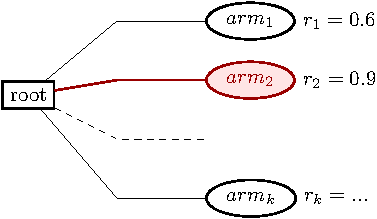
\includegraphics[scale=1.0]{onelevel-tree.pdf}\\
    \vspace{4em}
    a. search tree
  \end{minipage}
  \begin{minipage}[c]{0.5\linewidth}
    \centering
    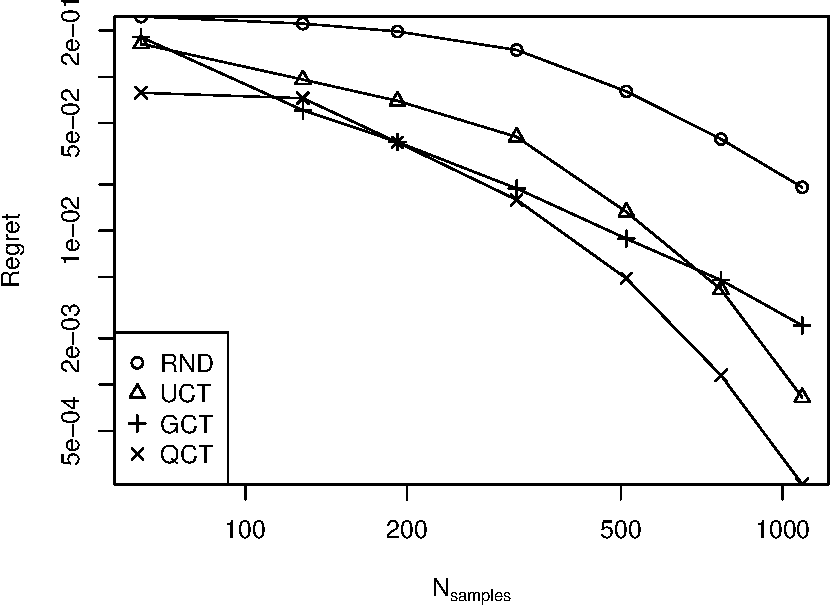
\includegraphics[scale=0.5]{flat-trilevel-k=64-uqb=8.pdf}\\
    b. regret vs. number of samples
  \end{minipage}
  \label{fig:mab-simple-regret}
  \caption{Simple regret in MAB}
\end{figure}

\subsection{Monte Carlo tree search}
\label{seq:emp-mcts}

The second set of experiments was performed on randomly generated
trees crafted in such a way that uniform random sampling selects a
direction at the root randomly. The degree of the root is a parameter of
the tree generator. The degree of all nodes at distance 1 from the
root is 2, and all nodes at distance 2 from the roots are leaves. The
average reward of two children of each node at distance 1 is
0.5. Thus, a uniform sampling scheme results in the same average reward for
all edges at the root, and an adaptive sampling scheme, such as UCT,
has to be used.

Figure~\ref{fig:mcts-regret} shows a sketch of the search tree
(Figure~\ref{fig:mcts-regret}.a) and the dependency of the regret vs. the
number of samples for trees with root degree 16
(Figure~\ref{fig:mcts-regret}.b) and 64 (Figure~\ref{fig:mcts-regret}.c). The
dependencies look differently from Multi-armed bandit instances, but
the algorithms exhibit a similar relative performance: either GCT or QCT
is always better than UCT, QCT dominates UCT everywhere
except for small numbers of instances. The advantage of QCT grows with
the number of arms.

\begin{figure}
  \begin{minipage}[c]{0.5\linewidth}
    \centering
    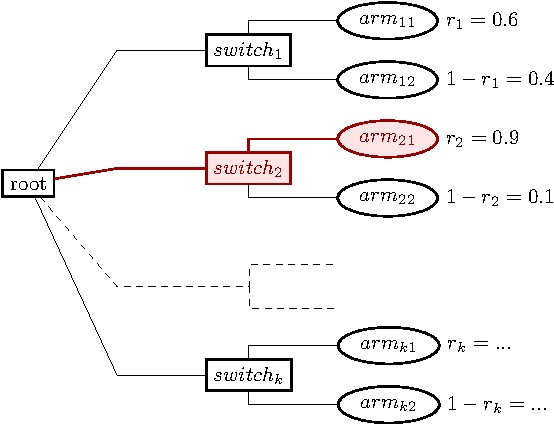
\includegraphics[scale=0.8]{twolevel-tree.pdf}\\
    a. search tree
  \end{minipage}
  \begin{minipage}[c]{0.5\linewidth}
    \centering
    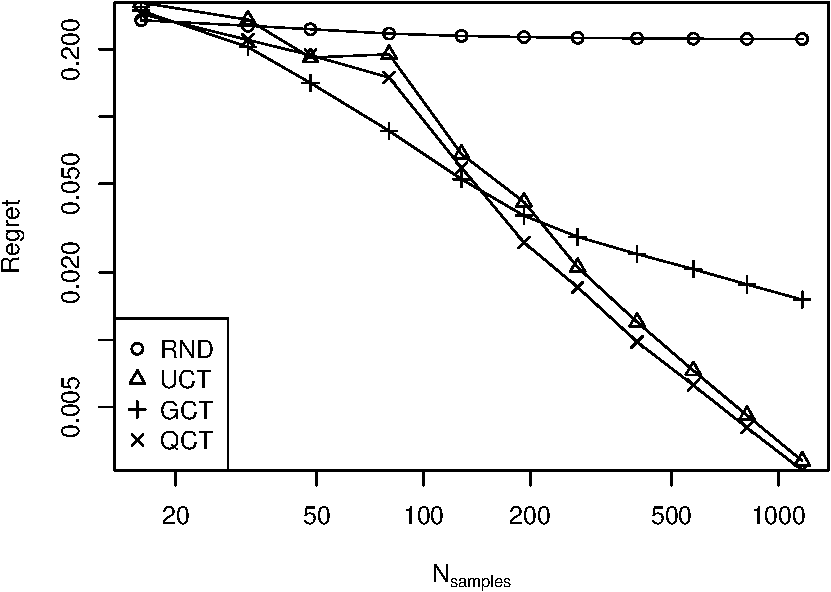
\includegraphics[scale=0.4]{tree-identity-k=16-uqb=8.pdf}\\ 
    b. 16 arms \\
    \vspace{1em}
    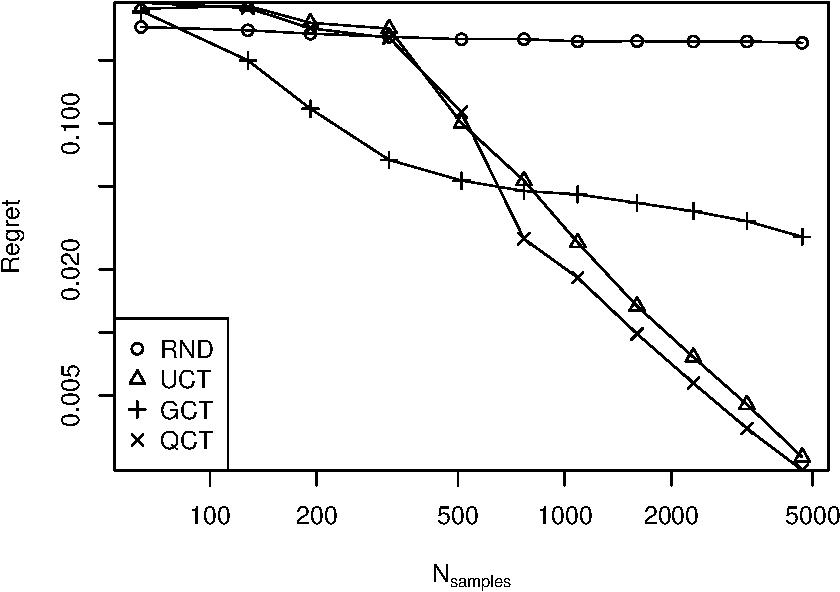
\includegraphics[scale=0.4]{tree-identity-k=64-uqb=8.pdf} \\
    c. 64 arms
 \end{minipage}
  \label{fig:mcts-regret}
  \caption{MCTS: a path to the best arm}
\end{figure}

\subsection{The sailing domain}
\label{seq:emp-sailing}

Figures~\ref{fig:sailing-cost-vs-nsamples}--\ref{fig:sailing-rcq-vs-factor}
show results of experiments on the sailing
domain. Figure~\ref{fig:sailing-cost-vs-nsamples} shows the regret
vs. the number of samples, computed for a range of values of
$C_p$. Figure~\ref{fig:sailing-cost-vs-nsamples}.a shows the median
cost, and Figure~\ref{fig:sailing-cost-vs-nsamples}.b --- the minimum
costs. UCT is always worse than either $\frac 1 2$-greedy (GCT) or QCT, and is sensitive to
the value of $C_p$: the median cost is much higher than the minimum
cost for UCT. For both $\frac 1 2$-greedy and QCT, the difference is
significantly less prominent.

\begin{figure}[t]
  \begin{minipage}[b]{0.5\linewidth}
    \centering
    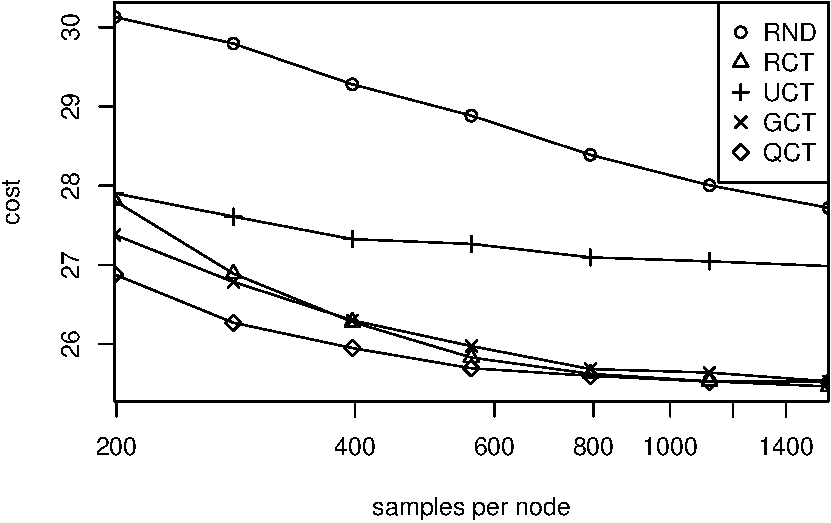
\includegraphics[scale=0.45]{costs-size=6-group=median.pdf}\\
    a. median cost
  \end{minipage}
  \begin{minipage}[b]{0.5\linewidth}
    \centering
    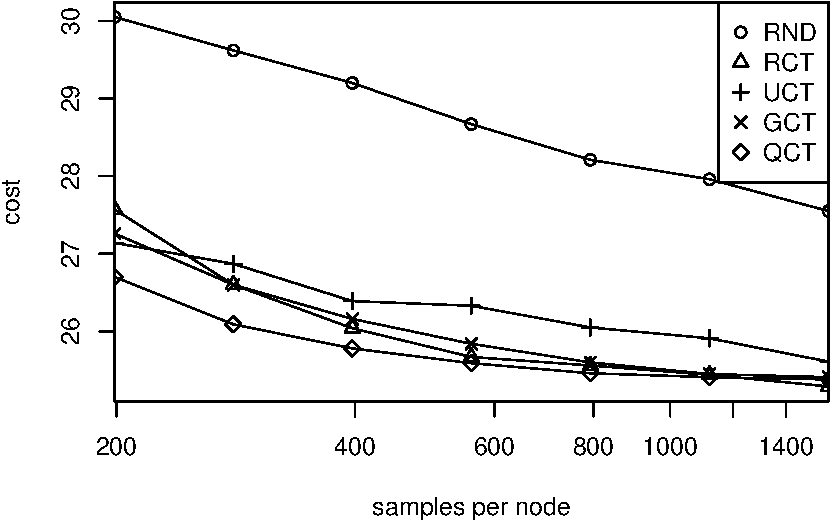
\includegraphics[scale=0.45]{costs-size=6-group=minimum.pdf}\\
    b. minimum cost
  \end{minipage}
  \caption{The sailing domain, $6\times 6$ lake, cost vs. number of rollouts}
  \label{fig:sailing-cost-vs-nsamples}
\end{figure}

Figure~\ref{fig:sailing-cost-vs-factor} shows the regret vs. the
exploration factor for different numbers of samples. QCT is always better than
UCT, and $\frac 1 2$-greedy is better than UCT expect for a small range of
values of the exploration factor $C_p$. 

\begin{figure}[t]
  \begin{minipage}[b]{0.5\linewidth}
    \centering
    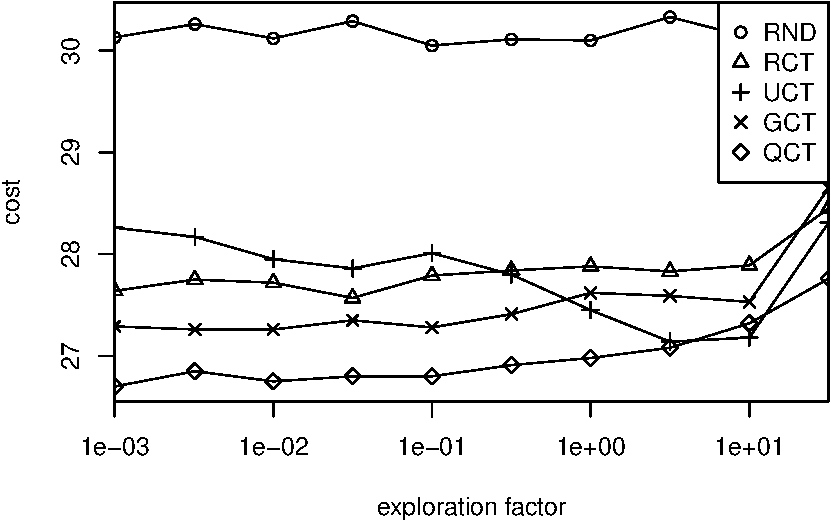
\includegraphics[scale=0.45]{costs-size=6-nsamples=199.pdf}\\
    a. 199 rollouts\\
    \vspace{1em}
    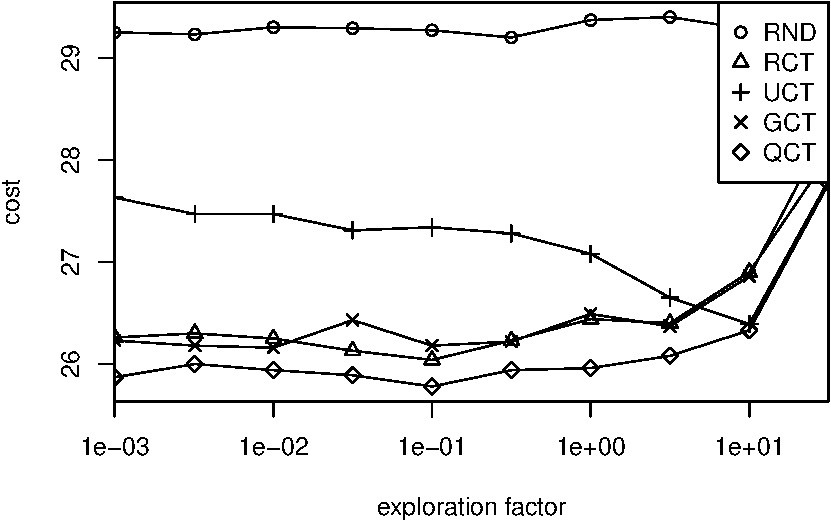
\includegraphics[scale=0.45]{costs-size=6-nsamples=397.pdf}\\
    b. 397 rollouts\\
  \end{minipage}
  \begin{minipage}[b]{0.5\linewidth}
    \centering
    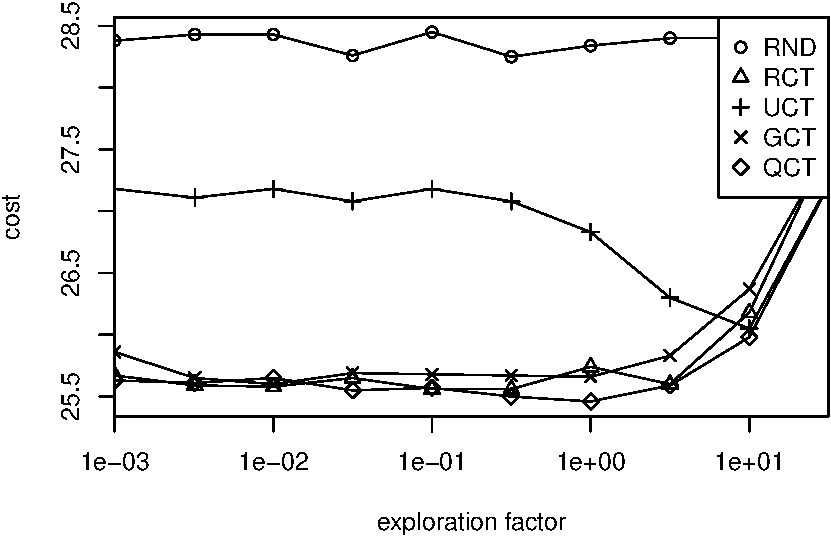
\includegraphics[scale=0.45]{costs-size=6-nsamples=793.pdf}\\
    c. 793 rollouts\\
    \vspace{1em}
    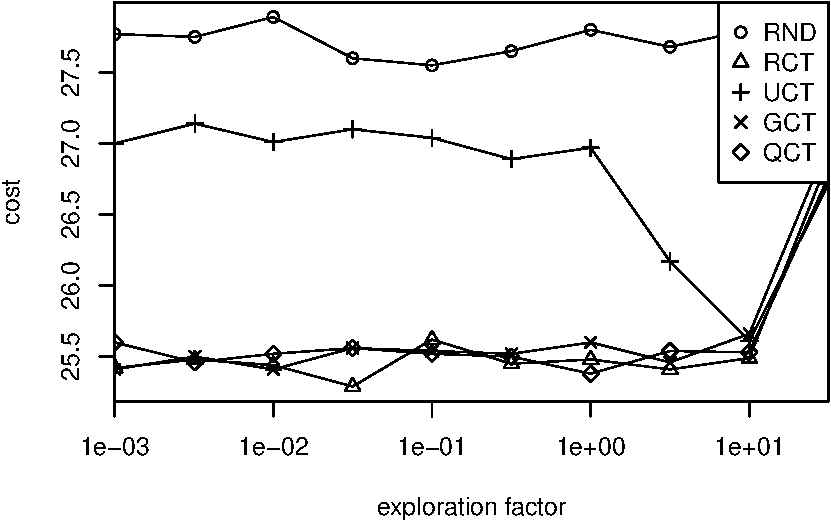
\includegraphics[scale=0.45]{costs-size=6-nsamples=1585.pdf}\\
    d. 1585 rollouts\\
  \end{minipage}
  \caption{The sailing domain, $6\times 6$ lake, cost vs. factor}
  \label{fig:sailing-cost-vs-factor}
\end{figure}


Figure~\ref{fig:sailing-lake-size} shows the cost vs. the exploration
factor for lakes of different sizes. The relative difference between
the sampling schemes becomes more prominent when the lake size
increases.

\begin{figure}[t]
  \begin{minipage}[b]{0.333\linewidth}
    \centering
    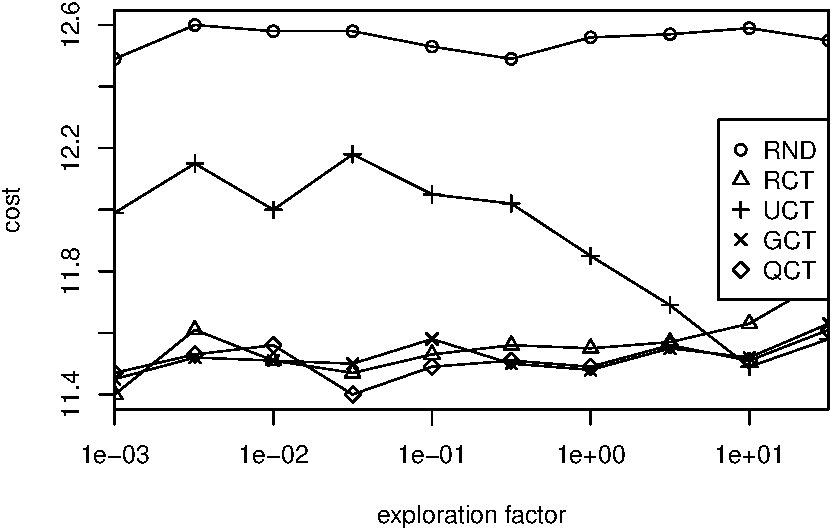
\includegraphics[scale=0.35]{costs-size=3-nsamples=397.pdf}\\
    a. $3\times 3$ lake
  \end{minipage}
  \begin{minipage}[b]{0.333\linewidth}
    \centering
    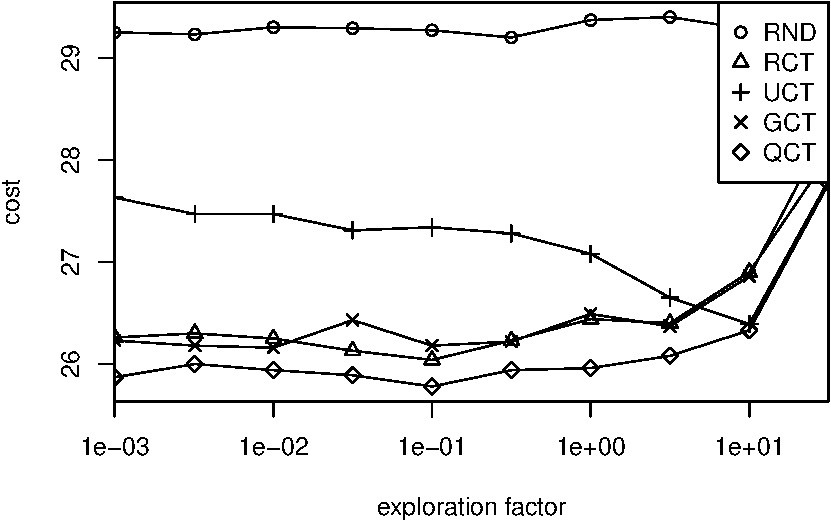
\includegraphics[scale=0.35]{costs-size=6-nsamples=397.pdf}\\
    b. $6\times 6$ lake
  \end{minipage}
  \begin{minipage}[b]{0.333\linewidth}
    \centering
    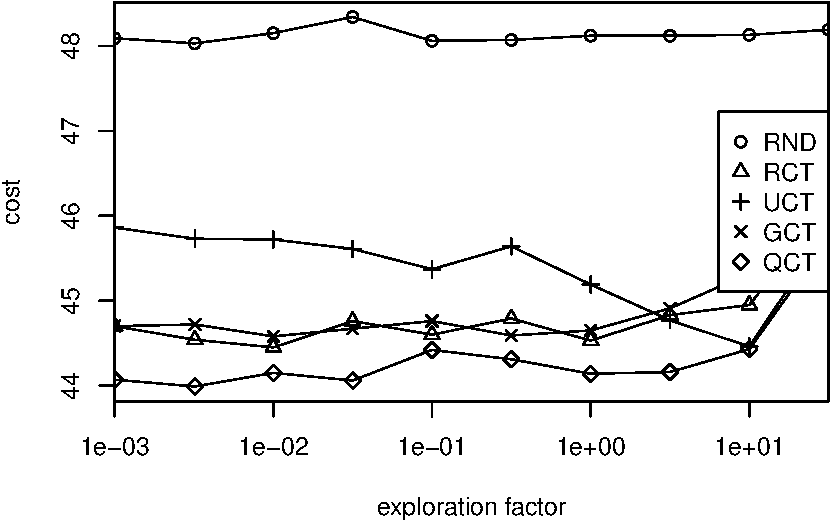
\includegraphics[scale=0.35]{costs-size=10-nsamples=397.pdf}\\
    b. $10\times 10$ lake
  \end{minipage}
  \caption{The sailing domain, 397 samples, cost vs. factor}
  \label{fig:sailing-lake-size}
\end{figure}

Figure~\ref{fig:sailing-rcq-vs-factor} compares QCT with UCT with a
different exploration factor at the root (CCT). $C_p$ for the rest of
the steps was chosen to ensure the best performance from earlier
experiments on the domain. Both algorithms exhibit similar dependency,
but as the number of samples grows, QCT achieves smaller average
regrets and is less sensitive to the choice of the value for $C_p$ at
the first step.

\begin{figure}[t]
  \begin{minipage}[b]{0.5\linewidth}
    \centering
    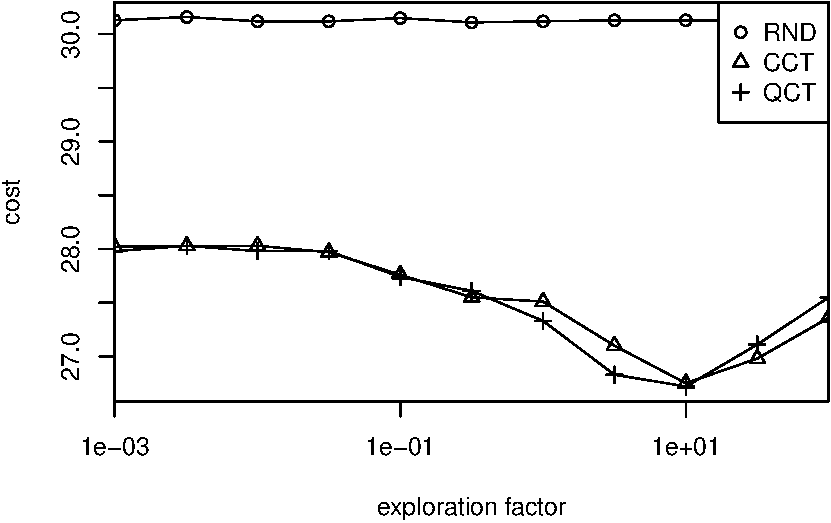
\includegraphics[scale=0.45]{rcq-size=6-nsamples=199.pdf}\\
    a. 199 rollouts\\
    \vspace{1em}
    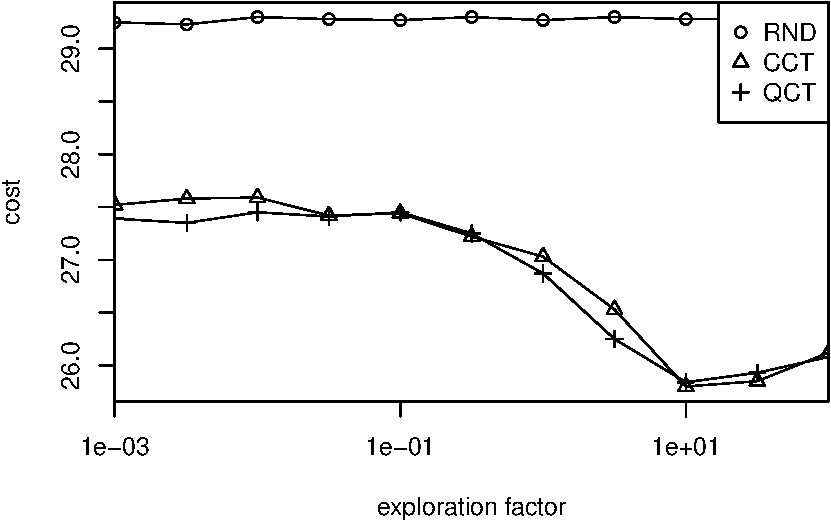
\includegraphics[scale=0.45]{rcq-size=6-nsamples=397.pdf}\\
    b. 397 rollouts\\
  \end{minipage}
  \begin{minipage}[b]{0.5\linewidth}
    \centering
    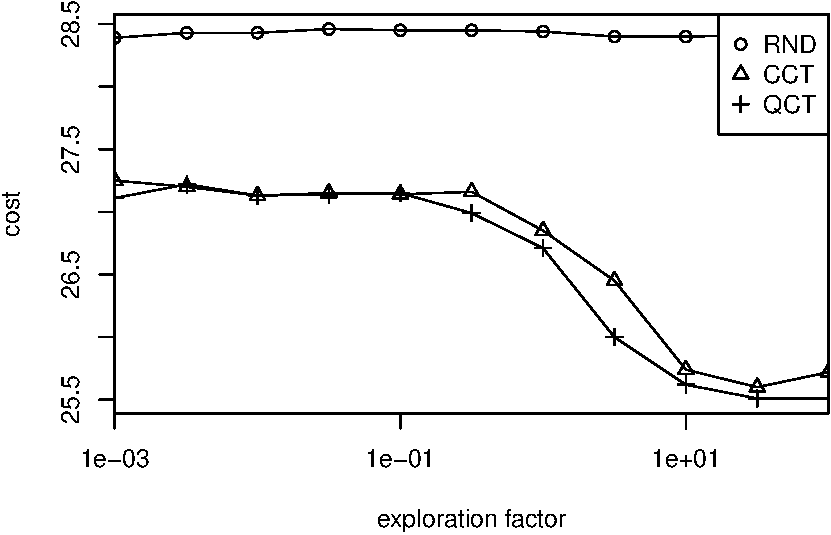
\includegraphics[scale=0.45]{rcq-size=6-nsamples=793.pdf}\\
    c. 793 rollouts\\
    \vspace{1em}
    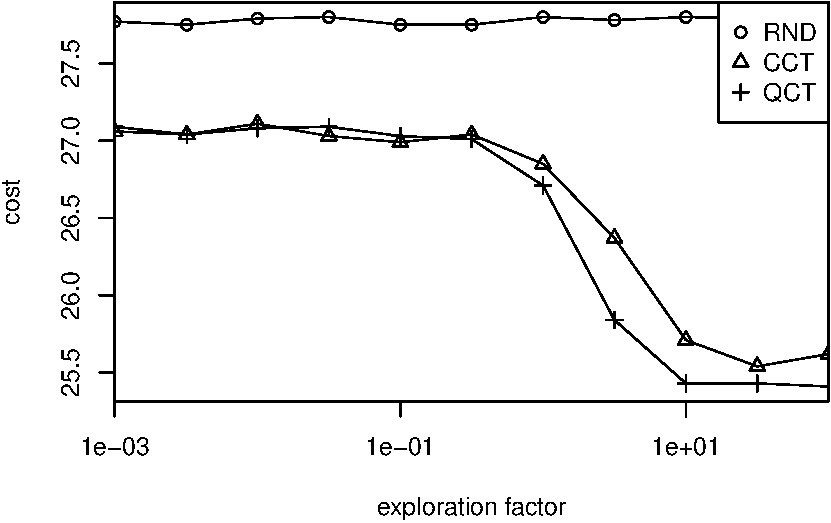
\includegraphics[scale=0.45]{rcq-size=6-nsamples=1585.pdf}\\
    d. 1585 rollouts\\
  \end{minipage}
  \caption{The sailing domain, log vs. sqrt, $6\times 6$ lake}
  \label{fig:sailing-rcq-vs-factor}
\end{figure}

\section{Summary and Future Work}

The Monte Carlo tree search algorithms presented in the paper differ
from UCT at the first step of the rollout, when the `simple' selection
regret is minimized instead of the cumulative regret. Both the
theoretical analysis and the empirical evaluation provide evidence for
better general performance of the proposed algorithms.

The improvement is inspired by the notion of value of information (VOI),
but VOI is used implicitly in the analysis of the algorithm, rather
than computed or learned explicitly in order to plan the rollouts. A
further improvement can be achieved by computing or estimating the VOI
of the rollouts and choosing a rollout that maximizes the VOI. Using VOI
to guide Monte Carlo sampling instead of relying on the sample means
of different actions  is particularly beneficial when different
actions have qualitatively different distributions: for example, when the
distribution variance varies significantly between the actions.

VOI of a rollout can be computed when the sample distribution of an
action is known up to the parameters, such as the normal distribution
with an unknown mean and/or variance. Alternatively, the value of
information can be estimated from the set of samples, and the need to
assume a particular shape of the distribution can be lifted. In one
realization of the latter approach the VOI of performing an action is
estimated as \emph{the value of perfect information learned from the outcome
of earlier samples of the action divided by the number of
samples}. Early experiments with this approach showed the best
performance for sets of Bernoulli arms, and even a more prominent
improvement for mixed arms (e.g. Bernoulli, triangularly distributed,
and fixed arms. Sample-based VOI estimation requires keeping more
information than an algorithm based only on the sample
mean, but the overhead is small and justified by the improvement.

\section*{Acknowledgments}

The research is partially supported by Israel
Science Foundation grant 305/09, by the Lynne and William Frankel
Center for Computer Sciences, and by the Paul Ivanier Center for
Robotics Research and Production Management.

\bibliographystyle{plain}
\bibliography{refs}


\end{document}
